\section{Concept Drift Components}
\label{sec:background_concept_drift_components}
Conventional machine learning primarily involves prediction and training/learning. However, learning under the concept drift paradigm introduces three additional critical steps as show in Fig. \ref{fig:concept-drift-components}: concept drift detection, drift understanding, and drift adaptation. Concept drift detection involves identifying changed points or change time periods to define and predict drift. Drift understanding delves into crucial aspects such as when the drift starts, how long it lasts, and where it occurs, providing indispensable insights for the subsequent adaptation step.  
The adaptation step, also referred to as the reaction step, plays a pivotal role in updating current learning models in response to concept drift. Three main approaches address various types of drift: Simple Retraining, Ensemble Retraining, and Model Adjusting. Drift detection employs various tools and algorithms, comparing old and fresh data chunks with statistical models based on data distribution. Techniques vary, with some utilizing a constant chunk length and others employing a variable length.
Drift understanding is essential for making well-informed decisions during the adaptation step. This involves calculating the necessary modifications in the trained model to adapt to new changes as shown in Fig. \ref{fig:concept-drift-understanding}. The severity region determines whether to generate a completely new model or make minimal adjustments to the existing one.

 
\begin{figure}[!ht]
    \centering
    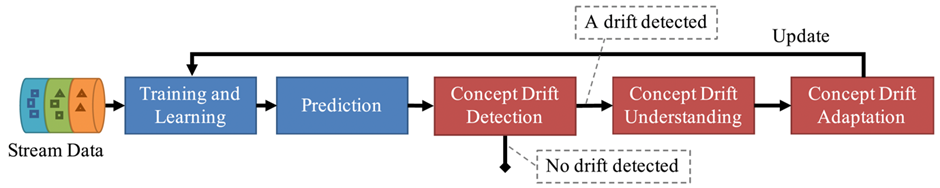
\includegraphics[width=.9\textwidth]{2_Background/figures/concept_drift_components.png}
    \caption{Main components of concept drift. \\ \textcolor{gray}{\fontsize{10}{0}\selectfont DOI: 10.1109/TKDE.2018.2876857}}

    \label{fig:concept-drift-components}
\end{figure}


%==============================[detection subsection]===============
\subsection{Concept Drift Detection}
Drift detection involves techniques and mechanisms to characterize and quantify concept drift by identifying change points or intervals \cite{liu2018making}. The general framework for drift detection consists of four stages:
\begin{itemize}
    \item \textbf{Stage 1 (Data Retrieval):} This stage focuses on retrieving data chunks from data streams. Given that a single data instance lacks sufficient information to infer the overall distribution \cite{lu2016concept}, organizing data chunks meaningfully is crucial for effective data stream analysis \cite{ramirez2017survey}.
    \item \textbf{Stage 2 (Data Modeling):} This optional stage abstracts the retrieved data, extracting key features that contain sensitive information impacting a system in case of drift. This stage may involve dimensionality reduction or sample size reduction to meet storage and online speed requirements \cite{liu2018making}.
    \item \textbf{Stage 3 (Test Statistics Calculation):} This stage involves measuring dissimilarity or estimating distance to quantify drift severity and generate test statistics for hypothesis testing. Defining an accurate and robust dissimilarity measurement remains a challenging aspect of concept drift detection. Test statistics can also be used for clustering evaluation \cite{silva2013data} and to determine dissimilarity between sample sets \cite{dries2009adaptive}.
    \item \textbf{Stage 4 (Hypothesis Test):} This stage employs a specific hypothesis test to assess the statistical significance of the change observed in Stage 3, such as the p-value. These tests determine drift detection accuracy by establishing statistical bounds for the test statistics from Stage 3. Without Stage 4, the acquired test statistics are meaningless for drift detection, as they cannot establish the drift confidence interval. Commonly used hypothesis tests include estimating the distribution of test statistics \cite{alippi2008just} \cite{gama2004learning}, bootstrapping \cite{bu2016pdf} \cite{venkatasubramanianinformation}, the permutation test \cite{lu2016concept}, and Hoeffding's inequality-based bound identification \cite{frias2014online}.
\end{itemize}

It is crucial to note that without Stage 1, the concept drift detection problem can be regarded as a two-sample test problem, examining whether the populations of two given sample sets are from the same distribution \cite{dries2009adaptive}. In other words, any multivariate two-sample test can be adopted in Stages 2-4 for detecting concept drift \cite{dries2009adaptive}. However, in cases where distribution drift may not be included in the target features, the selection of the target feature becomes critical for the overall performance of a learning system and poses a significant challenge in concept drift detection \cite{yamada2013change}.

%==============================[detection Understanding]===============
\subsection{Understanding Phase}
The extent of concept drift severity serves as a valuable criterion for selecting appropriate drift adaptation strategies. As shown in Fig. \ref{fig:concept-drift-understanding}, in a classification task where the drift's severity is minimal, resulting in only a marginal shift in the decision boundary within the new concept, adjusting the current learner through incremental learning proves sufficient. Conversely, when confronted with high severity in concept drift, wherein the decision boundary undergoes substantial changes, it might be more effective to discard the old learner and opt for retraining a new one rather than incrementally updating the existing learner. It's noteworthy to mention that despite some researchers highlighting the capability to articulate and quantify the severity of detected drift, this information is not yet widely integrated into drift adaptation practices.
The adaptation step offers three distinct ways to adapt the model. Simple Retraining involves training a new model using the most recent data, replacing the old model. Model Ensemble, the second approach, entails keeping and reusing existing models, which proves efficient when dealing with repeated instances of concept drift. The third approach, Model Adjusting, constructs a model that adapts flexibly from changed data, allowing partial updates when the original data distribution undergoes significant changes.

\begin{figure}[!ht]
    \centering
    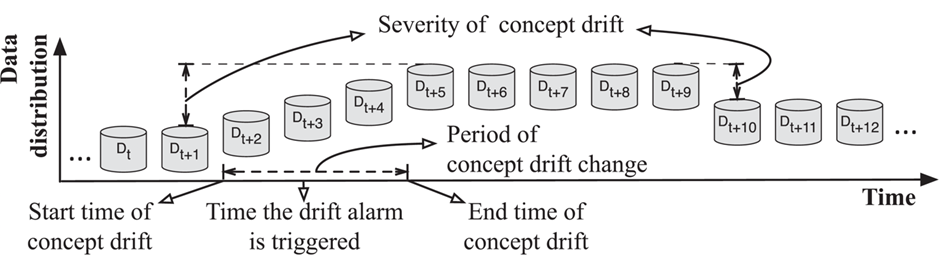
\includegraphics[width=.9\textwidth]{2_Background/figures/concept_drift_understanding.png}
    \caption{Understanding phase of concept drift. \\ \textcolor{gray}{\fontsize{10}{0}\selectfont DOI: 10.1109/TKDE.2018.2876857}}
    \label{fig:concept-drift-understanding}
\end{figure}

%==============================[Adaptation Adaptation]===============
\subsection{Adaptation Phase}
This section delves into strategies for updating existing learning models in response to drift, referred to as drift adaptation or reaction. The three primary categories of drift adaptation methods are simple retraining, ensemble retraining, and model adjusting, each tailored to address specific types of drift.

\begin{enumerate}[label=\Alph*.]
    \item \textbf{Simple Retraining} \\
    One way to respond to concept drift is by retraining a new model with the latest data, replacing the outdated model as shown in Fig.\ref{fig:concept-drift-adaptation}. This approach requires an explicit concept drift detector to determine when to retrain the current model. A window strategy is commonly used, preserving recent data for retraining and/or utilizing old data for distribution change tests. An example of this strategy is Paired Learners \cite{bach2008paired}, which employs two learners: the stable learner and the reactive learner. If the stable learner consistently misclassifies instances correctly classified by the reactive learner, indicating a new concept, the stable learner is replaced with the reactive learner. This method is straightforward, easy to implement, and adaptable at any point in the data stream.
    However, a trade-off arises when adopting a window-based strategy in determining an appropriate window size. A small window better reflects the latest data distribution, while a large window provides more data for training a new model. To address this challenge, the ADWIN algorithm \cite{bifet2007learning} dynamically adjusts sub window sizes based on the rate of change between two sub-windows, eliminating the need for users to predefine window sizes.
    Beyond direct model retraining, researchers have explored integrating the drift detection process with the retraining process for specific machine learning algorithms. DELM \cite{xu2017dynamic}, for instance, extends the traditional ELM algorithm, adapting to concept drift by dynamically adjusting the number of hidden layer nodes in response to increasing classification error rates, indicating a potential concept drift.
    Similarly, FP-ELM \cite{liu2016fp} introduces a forgetting parameter to the ELM model to adapt to drift conditions. A parallel version of the ELM-based method \cite{han2015efficient} has been developed for high-speed classification tasks under concept drift. OS-ELM \cite{soares2016adaptive}, an online learning ensemble of repressor models, integrates ELM using an ordered aggregation (OA) technique to address the challenge of defining the optimal ensemble size.
    In the realm of instance-based lazy learners for handling concept drift, the Just-in-Time adaptive classifier \cite{alippi2008just}  follows the "detect and update model" strategy, extending the traditional CUSUM test \cite{manly2000cumulative} to a pdf-free form for drift detection. When a concept drift is identified, old instances (beyond the last T samples) are removed from the case base. Advancements include extending this algorithm to handle recurrent concepts by considering and comparing the current concept to previously stored concepts \cite{silva2013data} \cite{alippi2008just}. NEFCS \cite{lu2016concept}, another KNN-based adaptive model, employs a competence model-based drift detection algorithm \cite{lu2016concept} to locate drift instances in the case base and distinguish them from noise instances. The redundancy removal algorithm, Stepwise Redundancy Removal (SRR), is developed to eliminate redundant instances uniformly, ensuring that the reduced case base retains sufficient information for future drift detection.
    

\begin{figure}[!ht]
    \centering
    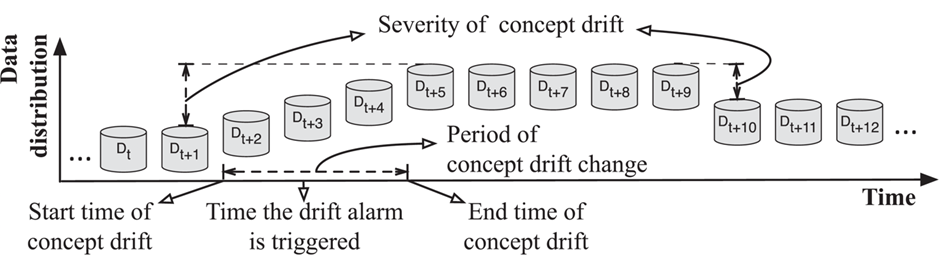
\includegraphics[width=.9\textwidth]{2_Background/figures/concept_drift_understanding.png}
    \caption{Approach for retraining a new model. \\ \textcolor{gray}{\fontsize{10}{0}\selectfont DOI: 10.1109/TKDE.2018.2876857}}
    \label{fig:concept-drift-adaptation}
\end{figure}





\item \textbf{Model Ensemble for Recurring Drift} \\
In recurring concept drift scenarios, preserving and reusing old models can be more efficient than retraining new ones for each recurrence, forming the basis for employing ensemble methods \cite{sun2018concept}. These methods, a focus in stream data mining research, consist of base classifiers with varied types or parameters. Their outputs, determined by specific voting rules, collectively predict new data. Various adaptive ensemble methods, extending classical ones or introducing adaptive voting rules, address the challenges of concept drift as shown in Fig. \ref{fig:concept-drift-ensemble}.
Classical ensemble methods like Bagging, Boosting, and Random Forests have been adapted for streaming data with concept drift. For instance, online Bagging \cite{oza2001experimental} uses each instance once, simulating batch mode bagging. Leveraging Bagging \cite{bifet2009new} employs ADWIN drift detection to replace the existing classifier with the worst performance when concept drift is detected.
 Adaptive boosting \cite{chu2004fast}, monitoring prediction accuracy through a hypothesis test, addresses concept drift, assuming classification errors on non-drifting data follow a Gaussian distribution. The Adaptive Random Forest (ARF) algorithm \cite{gomes2017adaptive} extends the random forest tree algorithm, incorporating concept drift detection (e.g., ADWIN) to decide when to replace an obsolete tree. A similar approach is seen in \cite{li2015learning}, using Beyond classical methods, novel ensemble methods with innovative voting techniques tackle concept drift. Dynamic Weighted Majority (DWM) \cite{kolter2007dynamic} adapts to drifts through weighted voting rules, managing base classifiers based on individual and global ensemble performance. Learn++NSE \cite{elwell2011incremental} addresses frequent classifier additions by weighting them based on prediction error rates.
 Specific types of concept drift are considered in specialized ensemble methods. Accuracy Update Ensemble (AUE2) \cite{brzezinski2013reacting} equally addresses sudden and gradual drift, using a batch mode weighted voting ensemble method. Optimal Weights Adjustment (OWA) \cite{zhang2008categorizing} achieves a similar goal with weighted instances and classifiers. Special cases, like class evolution, are considered in \cite{sun2016online}, while recurring concepts are handled by monitoring concept information \cite{gomes2013mining} \cite{gama2014survey} .Another method \cite{ahmadi2018modeling}, refines the concept pool for recurring concepts.
 
 \begin{figure}[!ht]
    \centering
    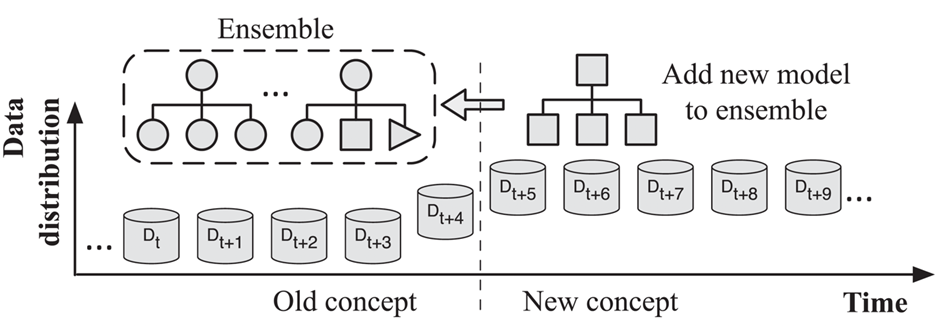
\includegraphics[width=.9\textwidth]{2_Background/figures/ensemble_update.png}
    \caption{Ensemble approach for the adaptation phase. \\ \textcolor{gray}{\fontsize{10}{0}\selectfont DOI: 10.1109/TKDE.2018.2876857}}
    \label{fig:concept-drift-ensemble}
\end{figure}




\item \textbf{Model Ensemble for Recurring Drift} \\
As Shown in Fig. \ref{fig:concept-drift-partial-update}, instead of retraining the entire model, an alternative is to construct a model with adaptive learning capabilities, allowing partial updates in response to changing data distributions \cite{pratama2015evolving}, as in Fig. \ref{fig:concept-drift-partial-update}. This is efficient when concept drift occurs in localized regions. Many techniques in this category use the decision tree algorithm, leveraging its ability to adapt to individual sub-regions.
VFDT \cite{domingos2000mining} is a foundational contribution for high-speed data streams, employing the Hoeffding bound for node splitting. VFDT processes each instance once, doesn't store instances, and has minimal maintenance costs. CVFDT \cite{hulten2001mining}, an extension, addresses concept drift by maintaining a sliding window of the latest data and replacing the original sub-tree with a better-performing alternative.
VFDTc \cite{hulten2001mining} enhances VFDT by handling numerical attributes and adapting to concept drift with node-level detection. Later extensions \cite{yang2012incrementally} \cite{yang2015countering} introduce an adaptive leaf strategy in VFDTc, selecting the best classifier from options like majority voting, Naive Bayes, and Weighted Naive Bayes. Recent studies \cite{rutkowski2012decision}\cite{rutkowski2014new} question VFDT's foundation, the Hoeffding bound, for non-independent variables in information gain. An alternative impurity measure is proposed in a new online decision tree model \cite{rutkowski2014new}, demonstrating its reflection of concept drift and potential use in CVFDT. IADEM-3 \cite{frias2016online} addresses Hoeffding bound concerns by computing the sum of independent random variables for drift detection and pruning.

 \begin{figure}[!ht]
    \centering
    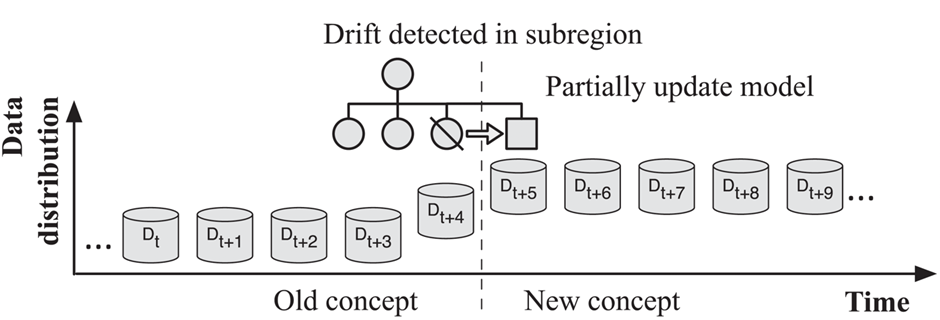
\includegraphics[width=.9\textwidth]{2_Background/figures/partial_update.png}
    \caption{Partial updating approach for the adaptation phase. \\ \textcolor{gray}{\fontsize{10}{0}\selectfont DOI: 10.1109/TKDE.2018.2876857}}
    \label{fig:concept-drift-partial-update}
\end{figure}
\end{enumerate}